\section{Vorlesung 11.05.2017}

\subsection{Teil 1: Populationsdynamik}
\textbf{Eindimensional:}\\
$\dot{x}=f(x), x(0)=x_{(0)}$\\
Fixpunkte: $\dot{x}=0=f(\hat{x})$\\
% pic 1

$x-\hat{x}=\epsilon \leftrightarrow x=\hat{x}+\epsilon$\\
\textcolor{red}{$\hat{x}=\dot{\epsilon}$?}\\
$\dot{x}=\dot{\epsilon}=f(x)=f(\hat{x}+\epsilon)$\\
durch Taylorreihe folgt: $\underbrace{f(\hat{x})}_{=0} + \frac{\delta f(\hat{x})}{\delta x} \cdot \epsilon + \text{Rest}(\epsilon^2)$\\
$\dot{\epsilon}=\frac{\delta f(\hat{x})}{\delta x}\cdot \epsilon$ für $|\epsilon|$ klein\\
$\epsilon(t)=e^{\frac{\delta f(\hat{x})}{\delta x}\cdot t} \cdot \epsilon(0)$\\
$\frac{\delta f(\hat{x})}{\delta x} < 0 \Rightarrow$ stabil $\hat{=}$ anziehend\\
$\frac{\delta f(\hat{x})}{\delta x} > 0 \Rightarrow$ instabil $\hat{=}$ abstoßend\\\\

\textbf{Mehrdimensional:}\\
DGL. System 1. Ordnung\\
$\dot{x_1}=f_1(x_1, x_2, ..., x_n)$\\
...\\
$\dot{x_n}=f_n(x_1, x_2, ..., x_n)$\\\\
\underline{Anfangsbedingungen (AB):}\\
$x_1(0)=\dot{x_1}$\\
...\\
$x_n(0)=\dot{x_n}$\\ \textcolor{red}{wo kommen die Punkte hin? $\dot{x_n}$ oder $x_{\dot{n}}$}\\\\

\underline{Fragen:}
\begin{enumerate}
	\item Existenz von Lösungen?
	\item Eindeutigkeit?
	\item Wie schaut die Lösung überhaupt aus?
\end{enumerate}

Betrachten unser DGL. System auf einem Gebiet $\Omega \subseteq R^n$\\
$f=(f_1 ... f_n)^T$\\
$f : x \mapsto f(x)$ Vektorfeld\\
$x \in \Omega, R^n $... n-dim Vektor von Änderungen\\

\underline{Lösung:}\\
% pic 2

\underline{Übungsaufgabe:} Visualisiere die Vektorfelder für Reuber-Beute Modelle\\\\

\underline{Annahme:} Vektorfeld f ist mindestens 1 mal stetig differenzierbar, d.h.\\
$\frac{\delta f_i}{\delta x_j}$ existiert auf ganz $\Omega$, sind auf ganz $\Omega$ stetig\\\\

$\Rightarrow$ Existenz: für jede Anfangsbedingung $x_0$ in $\Omega$ gibt es eine Zeitspanne $T(x_0)$ sodass $x(t|x_0)$ für alle $0 \leq t \leq T(x_0)$ existiert, eindeutig ist und $t \mapsto x(t|x_0)$ stetig ist\\

\textbf{Trajektorien kreuzen sich nie!}\\\\
% pic 3

Kreuzungspunkt nicht eindeutig $\Rightarrow$\\
$z_0=x_0(t_1)=y_0(t_2)$\\
$z(t|z_0)=x_0(t-t_1)=y_0(t-t_2)$\\
laut Eindeutigkeitssatz nicht möglich $\rightarrow$ Situation kann nicht vorkommen\\\\

Fixpunkte: $\hat{x} \in \Omega$ sodass $f(\hat{x})=0$\\

\subsubsection{Beispiel: Räuber-Beute-Modell}

\underline{Lotka-Volterra-Gleichung:} $f_i(x)=(r_i + \sum_{j} b_{ij} \cdot x_j) x_i$ mit\\\\
$r_i$ … Spezies-spezifische autonome Wachstumsrate\\
$\sum_{j} b_{ij} \cdot x_j$ … Interaktion mit allen (anderen) Spezies + intraspezifische Konkurenz $b_{ii}\cdot x_i$\\
$x_i$ … Wachstum proportional zur Populationsgröße\\

\underline{Fixpunkte in LV-Systemen:}\\
\begin{enumerate}
	\item Trivialer Fixpunkt:\\
	$x_1=x_2=…=x_n=0, \hat{x}=0 \Rightarrow$ alle Spezies ausgestorben
	\item innerer Fixpunkt: alle $x_i\neq 0$\\
	$f_i(x)=(r_i + (Bx)_i)x_i=0$ mit $(Bx)_i=\sum_{j} b_{ij} \cdot x_j$\\
	$\Leftrightarrow r_i + (Bx)_i = 0$\\
	$\Leftrightarrow Bx=-r$ (lineares GLS)\\
	$x=-B^{-1} \cdot r$
	\item Fixpunkte von Teilsystemen: $S=\{1,…,n\}$\\
	$A \subseteq S \rightarrow x_i=0 \text{ für } i \in S\backslash A$: verstorben, $x_i \neq 0 \text{ für } i \in A$
\end{enumerate}

\textbf{es existieren insgesamt $2^n$ mögliche Fixpunkte!}\\\\

\underline{\textbf{Status um Fixpunkte?}}\\
$\epsilon=x-\hat{x}, \epsilon_i=x_i-\hat{x_i}$\\
$\dot{\epsilon_i}=\dot{x_i}=f_i(x_1,…,x_n)=f_i(\hat{x}+\epsilon)=f_i(\hat{x_1}+\epsilon_1, … , \hat{x_n}+\epsilon_n)$\\
Taylorreihenentwicklung: $=f_i(\hat{x_1}, … , \hat{x_n}) + \displaystyle  \sum_{k} \frac{\delta f_i(\hat{x})}{\delta x_k} \cdot \epsilon_k + \text{Rest}(\epsilon^2)$\\
für $|\epsilon|$ sehr klein folgt:\\\\
\underline{Jacobimatrix} $J_{ik}:=\displaystyle \sum_{k} \frac{\delta f_i(\hat{x})}{\delta x_k}$\\\\
$\epsilon_i=(J_{\epsilon})_i$ zeitliche Entwicklung der Störung $\epsilon \Rightarrow \dot{\epsilon}=J(\hat{x}) \cdot \epsilon$\\

Das Verhalten von $\dot{x} = f(x)$ wird in der Nähe einer Fixpunktes $\hat{x}$ durch die Linearisierung $\dot{\epsilon} = J(\hat{x}) \cdot \epsilon$ beschrieben.\\

$\Rightarrow$ müssen verstehen, wie die Lösung von linearen DGL-Systemen aussehen\\
$\dot{x}=Ax, x \in R^n, A \in R^{n,n}$\\\\
\textbf{1. Dimension:}\\
$\dot{x}=a \cdot x \Rightarrow x(t)=e^{a \cdot t} \cdot x_0$\\
Formale Lösung in $R^n: x(t)=exp(t \cdot A) \cdot x_0$\\
Darstellung Exponentialfunktion Matrix:\\
Zahl: $e^a=1+\frac{1}{1!}a^1 + \frac{1}{2!}a^2 + …$\\\\
$exp(A):= \displaystyle \sum_{k=0}^{\infty} \frac{1}{k!} A^k$\\\\
$[exp(A)]_{ij}= \underbrace{\sum_{k=0}^{\infty} \frac{1}{k!} [A^k]_{ij}}_{\text{konvergiert für alle A}}$\\\\
$\Rightarrow exp(t \cdot A) = \displaystyle  \sum_{k=0}^{\infty} \frac{1}{k!} (t \cdot A)^k =  \displaystyle \sum_{k=0}^{\infty} \frac{t^k}{k!} A^k$\\\\
$\Rightarrow \frac{d}{dt} [exp(t \cdot A)]_{ij}=\displaystyle \sum_{k=0}^{\infty} \underbrace{\frac{dt^k}{dt}}_{k \cdot t^{k-1}} \cdot \frac{1}{k!} [A^k]_{ij}$\\\\
$=\displaystyle \sum_{k=0}^{\infty} t^{k-1} \cdot \underbrace{\frac{k}{k!}}_{k \cdot (k-1)!} [A^k]_{ij}$\\\\
$=\displaystyle \sum_{k=0}^{\infty} \frac{1}{(k-1)!} \cdot t^{k-1} [A^k]_{ij}$\\\\
mit $k-1=l$ folgt: $\displaystyle \sum_{l=0}^{\infty} \frac{1}{l!} \cdot t^l [A^{l+1}]_{ij}$\\\\
$\Rightarrow \frac{d}{dt} exp(t \cdot A)=\displaystyle \sum_{l=0}^{\infty} \frac{t^l}{l!} \cdot A^{l+1} = A \displaystyle \sum_{l=0}^{\infty} \underbrace{\frac{t^l}{l!} \cdot A^l}_{exp(t \cdot A)}=A \cdot exp(t \cdot A)$\\\\

$\dot{x} = A \cdot x \Rightarrow$ Ansatz:\\
$x(t)=exp(t \cdot A) \cdot x_0$\\
$\dot{x}(t)=A \underbrace{\cdot exp(t \cdot A) \cdot x_0}_{x(t)}$\\
$\Rightarrow x(t)=exp(t \cdot A) \cdot x_0$ löst tatsächlich die lineare DGL\\\\

\underline{Spezialfall:} Matrix A ist eine Diagonalmatrix\\

$A = 
\begin{pmatrix}
 \lambda_1 & \cdots & 0 \\
 \vdots  & \ddots & \vdots  \\
 0 & \cdots & \lambda_n
\end{pmatrix}
\Rightarrow
A^k = 
\begin{pmatrix}
 \lambda_1^k & \cdots & 0 \\
 \vdots  & \ddots & \vdots  \\
 0 & \cdots & \lambda_n^k
\end{pmatrix}$
\\\\

$\displaystyle \sum_{k=0}^{\infty} \frac{1}{k!} \cdot A^k=\displaystyle  \sum_{k=0}^{\infty} \frac{1}{k!} \cdot  
\begin{pmatrix}
 \lambda_1^k & \cdots & 0 \\
 \vdots  & \ddots & \vdots  \\
 0 & \cdots & \lambda_n^k
\end{pmatrix} = 
\begin{pmatrix}
 \sum_{k=0}^{\infty} \frac{1}{k!} \cdot \lambda_1^k & \cdots & 0 \\
 \vdots  & \ddots & \vdots  \\
 0 & \cdots & \sum_{k=0}^{\infty} \frac{1}{k!} \cdot \lambda_n^k
\end{pmatrix} = 
\begin{pmatrix}
 e^{\lambda_1} & \cdots & 0 \\
 \vdots  & \ddots & \vdots  \\
 0 & \cdots & e^{\lambda_n}
\end{pmatrix}
$
\\\\

$\Rightarrow x(t)=exp(tA)x_0$?\\
$x_i(t)=\sum_{j} [exp(tA)]_{ij} \cdot x_{\mathring{j}} = \sum_{j} e^{t \cdot \lambda_j} \cdot \delta_{ij} \cdot x_{\mathring{j}}$\\
mit $x_{\mathring{j}}=$j-Koordinate der $A_iB_i$, $\delta_{ij}$=Kronecker-Delta \textcolor{red}{was bedeutet $\mathring{j}$?}\\

$x_i(t)=e^{t \lambda_i} \cdot x_{\mathring{j}}$
\\\\
$x_i(t) \rightarrow 0$ wenn $\lambda_i < 0$ stabile Richtung\\
$x_i(t) \rightsquigarrow \pm \infty$ wenn $\lambda_i > 0$ instabile Richtung\\\\
wenn alle Richtungen stabil: Senke\\
wenn alle Richtungen instabil: Quelle\\
sonst: Sattelpunkt\\

\underline{Was wenn Jacobimatrix nicht diagonal?}\\
Eigenwerte und Eigenvektoren\\
$Au=\lambda u \leftarrow u\neq 0$ Eigenvektor von A zum Eigenwert $\lambda$\\
$Au^{(j)}=\lambda_j u^{(j)}$\\
$U \cdot A \rightarrow A=
\begin{pmatrix}
 x_1 & \cdots & 0 \\
 \vdots  & \ddots & \vdots  \\
 0 & \cdots & x_n
\end{pmatrix}
$

$A \underbrace{[u^{(1)}, … , u^{(n)}]}_{*} = [\lambda_1 u^{(1)}, … , \lambda_n u^{(n)}]$\\
*… U-Matrix deren Spalten die Eigenvektoren von A sind\\\\

$A \cdot U = U \cdot A$ vorausgesetzt es gibt n linear unabhängige Eigenwerte von A\\
$U^{-1} exp(tA) U = U^{-1} \sum_{k=0}^{\infty} \frac{t^k}{k!} A^k U = U^{-1} \sum_{k=0}^{\infty} \frac{t^k}{k!} U A^k = \underbrace{U^{-1} U}_{I} \sum_{k=0}^{\infty} \frac{t^k}{k!} A^k$\\
$= exp(tA)=e^{tA}$
\\\\

$x(t)=exp(tA) \cdot x_0 = U exp(tA) U^{-1} \cdot x_0$\\
neue Koordinate: $y:=U^{-1}x \Leftrightarrow x=U \cdot y$\\
$\dot{y}=U^{-1} \dot{x} = U^{-1} Ax = \underbrace{U^{-1} \cdot A \cdot U}_{*} \cdot y = Ay$\\\\
* wenn A symmetrisch, dann gibt es n linear unabhängige Eigenvektoren, die sind sogar orthogonal $U^{-1}=U^T$ alle Eigenwerte $\lambda_i \in R$\\\\

\textcolor{red}{hier fehlt was im Skript von Christian}\\\\

Eigenwerte i. A. nicht reell:\\
macht nix, nehmen Eigenwerte über komplexe Zahlen\\
für jeden Eigenwert $\lambda=Re \lambda + i \cdot Im \lambda$ ist auch konjugiert komplexe Zahl $\lambda=Re \lambda - i \cdot Im \lambda$ ein Eigenwert\\\\

Satz von Moivre: $e^{t \lambda} = e^{t RE \lambda} \cdot e^{i t Im \lambda} = e^{t Re \lambda} (cos t Im \lambda + i sin t Im \lambda)$\\
$e^{t \overline{\lambda}} = e^{t RE \lambda} \cdot e^{- i t Im \lambda} = e^{t Re \lambda} (cos t Im \lambda - i sin t Im \lambda) \leftarrow$ Wirbel\\\\

$\lambda_i$ … reell in diese Eigenrichtung $u_i e^{t \lambda_i}$\\
$\lambda_i, \overline{\lambda_i}$ … Paar von konjugiert komplexen Eigenwerten dann gibt es 2D-Ebene, in der \\
$y_{1,2}(t)=e^{t Re \lambda} \cdot cos t Im \lambda$\\\\

% pic 3

Allgemeiner Fall: Stabilität durch $Re \lambda_i$ gegeben.\\
$Re \lambda_i < 0$ anziehende Richtung\\
$Re \lambda_i > 0$ abstoßende Richtung\\
Quelle: $Re \lambda_i > 0$ für alle i\\
Senke: $Re \lambda_i < 0$ für alle i\\
Sattelpunkt: sowohl $Re \lambda_i < 0$ als auch $Re \lambda_i > 0$ existieren.
\\\\
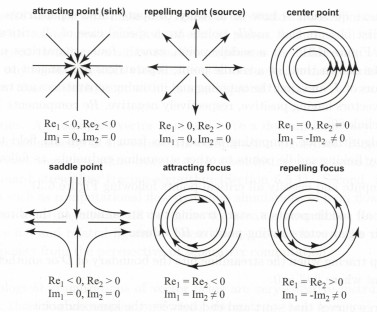
\includegraphics[scale=1.750]{lectures/170511/pix/critical_points}

\subsection{Teil 2: Diskussion zu den Vorträgen beim mitteldeutschen Bioinformatik-Meeting 2017}